\section{Đề xuất cải tiến}
\subsection{Cải tiến mô hình}

\incident Dựa vào tính khả thi của mô hình, data thu thập từ các hành động sẽ được reshape và tích hợp vào mô hình (không sử dụng bộ dữ liệu có sẵn trước đó), đảm bảo rằng quá trình reshape dữ liệu được thực hiện một cách chính xác và phù hợp với đầu vào của mô hình. 

\incident Mô hình cũng sẽ được phát triển thêm chức năng học chuyển tiếp để mô hình có khả năng học từ dữ liệu mới một cách hiệu quả Sử dụng trọng số đã được học trước đó từ mô hình để tận dụng thông tin học được từ dữ liệu cũ.

\incident Phát triển chức năng lưu và load model để giữ cho mô hình được duy trì và sử dụng lại một cách thuận tiện. Lưu trữ trọng số, cấu trúc mô hình và thông tin huấn luyện để có thể sử dụng lại mô hình một cách linh hoạt.

\incident Cải thiện độ chính xác hơn của model (độ chính xác hiện tại đạt khoảng 91\% dựa trên bộ dữ liệu có sẵn) mục tiêu đạt khoảng 95\%, tiếp tục tối ưu hóa mô hình để cải thiện độ chính xác. Thử nghiệm với các siêu tham số khác nhau, kiến trúc mạng nơ-ron, hoặc kỹ thuật tăng cường dữ liệu để nâng cao hiệu suất.


\incident Thực hiện giám sát kỹ thuật huấn luyện, đảm bảo rằng mô hình không bị overfitting hoặc underfitting.

\subsection{Cải tiến module cảm biến}
\incident Với thiết kế hiện tại của nhóm thì thiết bị chỉ có thể lấy dữ liệu về độ cong hay góc độ của ngón tay nên còn nhiều hạn chế khi nhận diện các cử chí phức tạp hơn như cử động ngón tay kết hợp với các hành động xoay, di chuyển bàn tay, cổ tay... Vì thế nhóm đề xuất sẽ sử dụng thêm các cảm biến gia tốc và con quay hồi chuyển. Hình \ref{fig:MPU6050} dưới đây là ví dụ minh họa cho một module cảm biến tích hợp gia tốc và con quay hồi chuyển MPU 6050.
\begin{figure}[H]
    \centering
    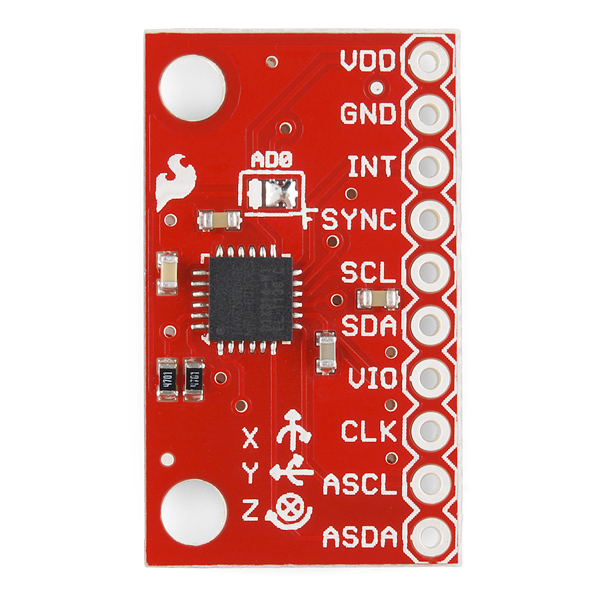
\includegraphics{Images/Theoretical basis/MPU6050.jpg}
    \caption{Module cảm biến tích hợp MPU6050}
    \label{fig:MPU6050}
\end{figure}
\incident Module cảm biến MPU6050 có khả năng đo trị số gia tốc trên cả 3 trục (X, Y, Z) giúp ta đo độ tăng tốc, giảm tốc của bàn tay khi cử động. Ngoài ra module còn có khả năng đo góc quay hoặc vận tốc góc trên các trục quay. Bằng việc đồng thời kết hợp các giá trị đo lường từ các cảm biến Flex với việc đọc và xử lý các giá trị từ module cảm biến MPU6050 sẽ giúp tăng khả năng nhận diện các cử động của cả bàn tay trong không gian ba chiều một cách chính xác hơn, tăng thêm được tiềm năng ứng dụng của đề tài.

\subsection{Module giao tiếp ngoại vi}
\incident Việc truyền dãn dữ liệu đọc được từ các thiết bị cảm biến về module nhận dạng cử chỉ bàn tay hiện tại được thực hiện qua kênh truyền có dây nên còn nhiều bất cập trong quá trình sử dụng thiết bị. Vì thế nhóm sẽ đề xuất thay thế kênh truyền có dây sang kênh truyền không dây thông qua Bluetooth hay WiFi để thuận tiện hơn khi sử dụng và góp phần tích hợp vào các hệ thống thông minh như nhà thông minh, thiết bị y tế thông minh,..
